\providecommand{\relativeRoot}{../..}
\documentclass[\relativeRoot/main.tex]{subfiles}
\graphicspath{
	{\relativeRoot/figures/}
    {\subfix{./figures/}}
}


\begin{document}

\section{Styling, Layout and Design}
\label{sec:lyprox:design}

Conceptually, the described online interface still fulfills the same purpose as the prototype shown in \cref{fig:lyprox:pouymayou_gui}. The new Django-based implementation has -- over the initial development period -- added a few more options for filtering the cohorts and how to treat multiple diagnoses per patient. Most visually striking, however, might be the overhauled visuals. The original prototype used the Python library \superhref{https://kivy.org}{Kivy} to run and render the \gls{gui}, which means the appearance is adjusted in the interface's code. \inlinelyproxlogo{}, on the other hand, only serves \acrshort{html} pages which are styled on the client side using the \acrshort{css} code delivered with it. This has the disadvantage that we could not easily transfer the appearance of the prototype to the online interface, but it makes setting up a modern, responsive and professionally looking web page very straightforward: There exists an abundance of \acrshort{css} frameworks that provide pre-defined and carefully designed building blocks that can quickly be combined and adapted to one's needs. So, to create a visually appealing \gls{gui}, it is sufficient to choose a \acrshort{css} framework, customize it to match the desired appearance and send it alongside the interface's \acrshort{html} responses.

We used the popular free and open source \acrshort{css} framework \superhref{https://bulma.io}{Bulma} \cite{thomas_bulma_2021}, which is published under MIT license. Very little \acrshort{css} knowledge is required to employ it effectively, but it is still heavily customizable and extensible, making it a safe choice for further development and potential design changes in the future.

Because we find the appearance of most default Bulma elements and components very appealing, we only customized the standard colors. For those, we chose the corporate design colors of the \gls{usz}. Initially, we decided to use them because we planned to host the website under an official \gls{usz} domain and on dedicated hardware from our institution. However, at the time of writing we were not provided with a URL or server by the \gls{usz}, so as of now \inlinelyproxlogo{} is hosted externally and under our own domain. Nonetheless, we find the \gls{usz} color scheme pleasing and modern-looking, so we kept it.

In \cref{fig:lyprox:plain_vs_bulma} we show a side-by-side comparison of a very simple \acrshort{html} page with and without the custom Bulma \acrshort{css} we also use for \inlinelyproxlogo{}. Notably, Bulma is agnostic to the type of \acrshort{html} tag. This can be seen in \cref{fig:lyprox:bulma}, where the title ``Bulma Demo'' corresponds to a normal \texttt{<p>} paragraph. Bulma's styling is always applied to class definitions of \acrshort{html} tags. In this case \texttt{<p class="title">} causes the larger font face, while the color depends on the parent \acrshort{html} element and its background color (see \cref{fig:lyprox:bulma}). This allows for a separation of form and function. E.g., a link \texttt{<a href="https://lyprox.org" class="button">} will look exactly the same as a submit button \texttt{<button type="submit" class="button">} when styled with Bulma, but might serve entirely different purposes.

\begin{figure}
    \begin{subfigure}[b]{0.48\textwidth}
        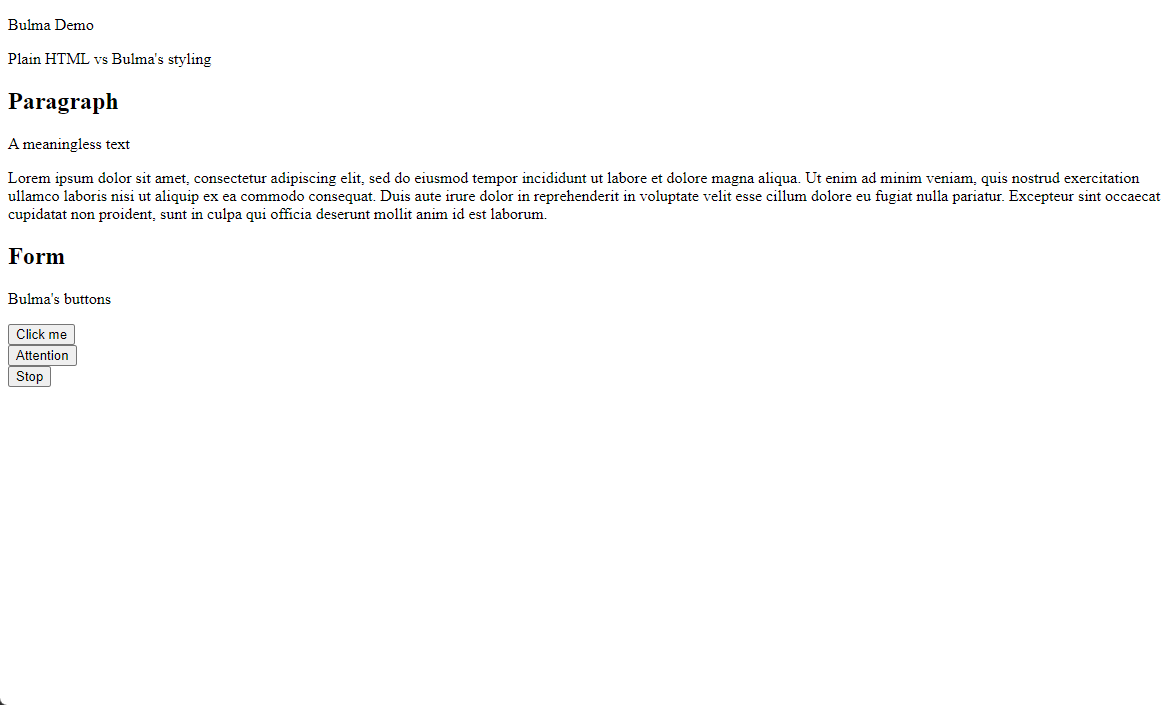
\includegraphics[width=\textwidth, frame]{figures/demo_without_bulma.png}
        \caption[
            Plain demo HTML document
        ]{
            Plain \acrshort{html} document for demonstration purposes, containing titles, a paragraph and three buttons.
        }
        \label{fig:lyprox:plain}
    \end{subfigure}
    \hfill
    \begin{subfigure}[b]{0.48\textwidth}
        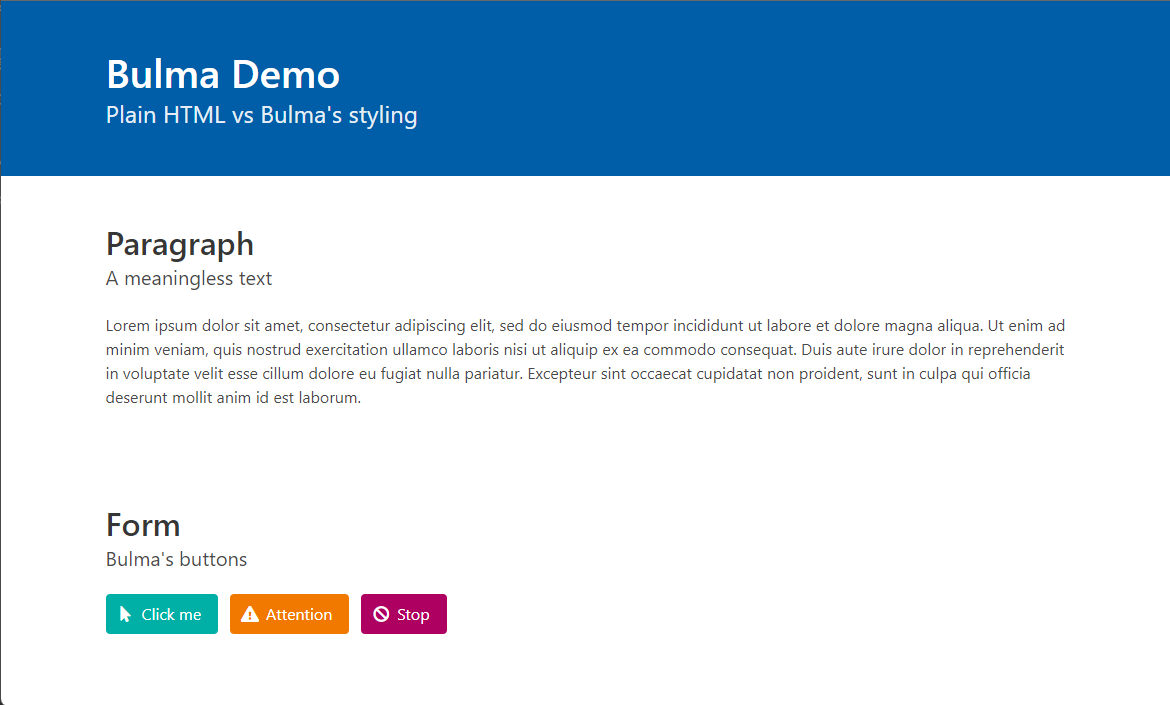
\includegraphics[width=\textwidth, frame]{figures/demo_with_bulma.png}
        \caption[
            HTML demo document with Bulma styling
        ]{
            The same \acrshort{html} document with Bulma \acrshort{css} styling with a color scheme matching the \gls{usz} corporate design.
        }
        \label{fig:lyprox:bulma}
    \end{subfigure}
    \caption[Plain HTML vs HTML plus CSS styling]{
        Comparison of how the same \acrshort{html} code gets rendered by a modern browser with and without \acrshort{css} styling.
    }
    \label{fig:lyprox:plain_vs_bulma}
\end{figure}

Besides Bulma's \acrshort{css}, we also use \superhref[\faIcon{font-awesome-flag}~]{https://fontawesome.com}{Font Awesome Free} (version 5) \cite{noauthor_font_2022} as a provider of icons. It allows the free use of 1,608 icons under the license \faIcon{creative-commons}\faIcon{creative-commons-by} \gls{cc-by} to make interface elements more visually appealing and familiar looking. Moreover, Bulma explicitly supports adding Font Awesome icons to many of its core elements. Their icons are also used throughout this thesis to provide visual cues, e.g. in the contribution boxes.

\end{document}
